\chapter{System Organization}
The entire architecture can be split into three parts: Memory transfer of packets to the GPU, Analysis on the GPU and Transfer results back to the CPU.

\section{Memory transfer of packets to the GPU}
The CPU captures the packets using the APIs provided by the packet capture library LibPCAP.  The packet capture library abstracts the packet capture process and provides a mechanism to capture packets which are send to another host machine. The library also provides a mechanism to read packets from a saved file. Due to the overhead associated with transferring data from CPU to GPU, it is better to save the packets into a buffer and transfer them.
The system is divided into many components. The diagram below shows the connection between these components.


\begin{figure}
	\centering
	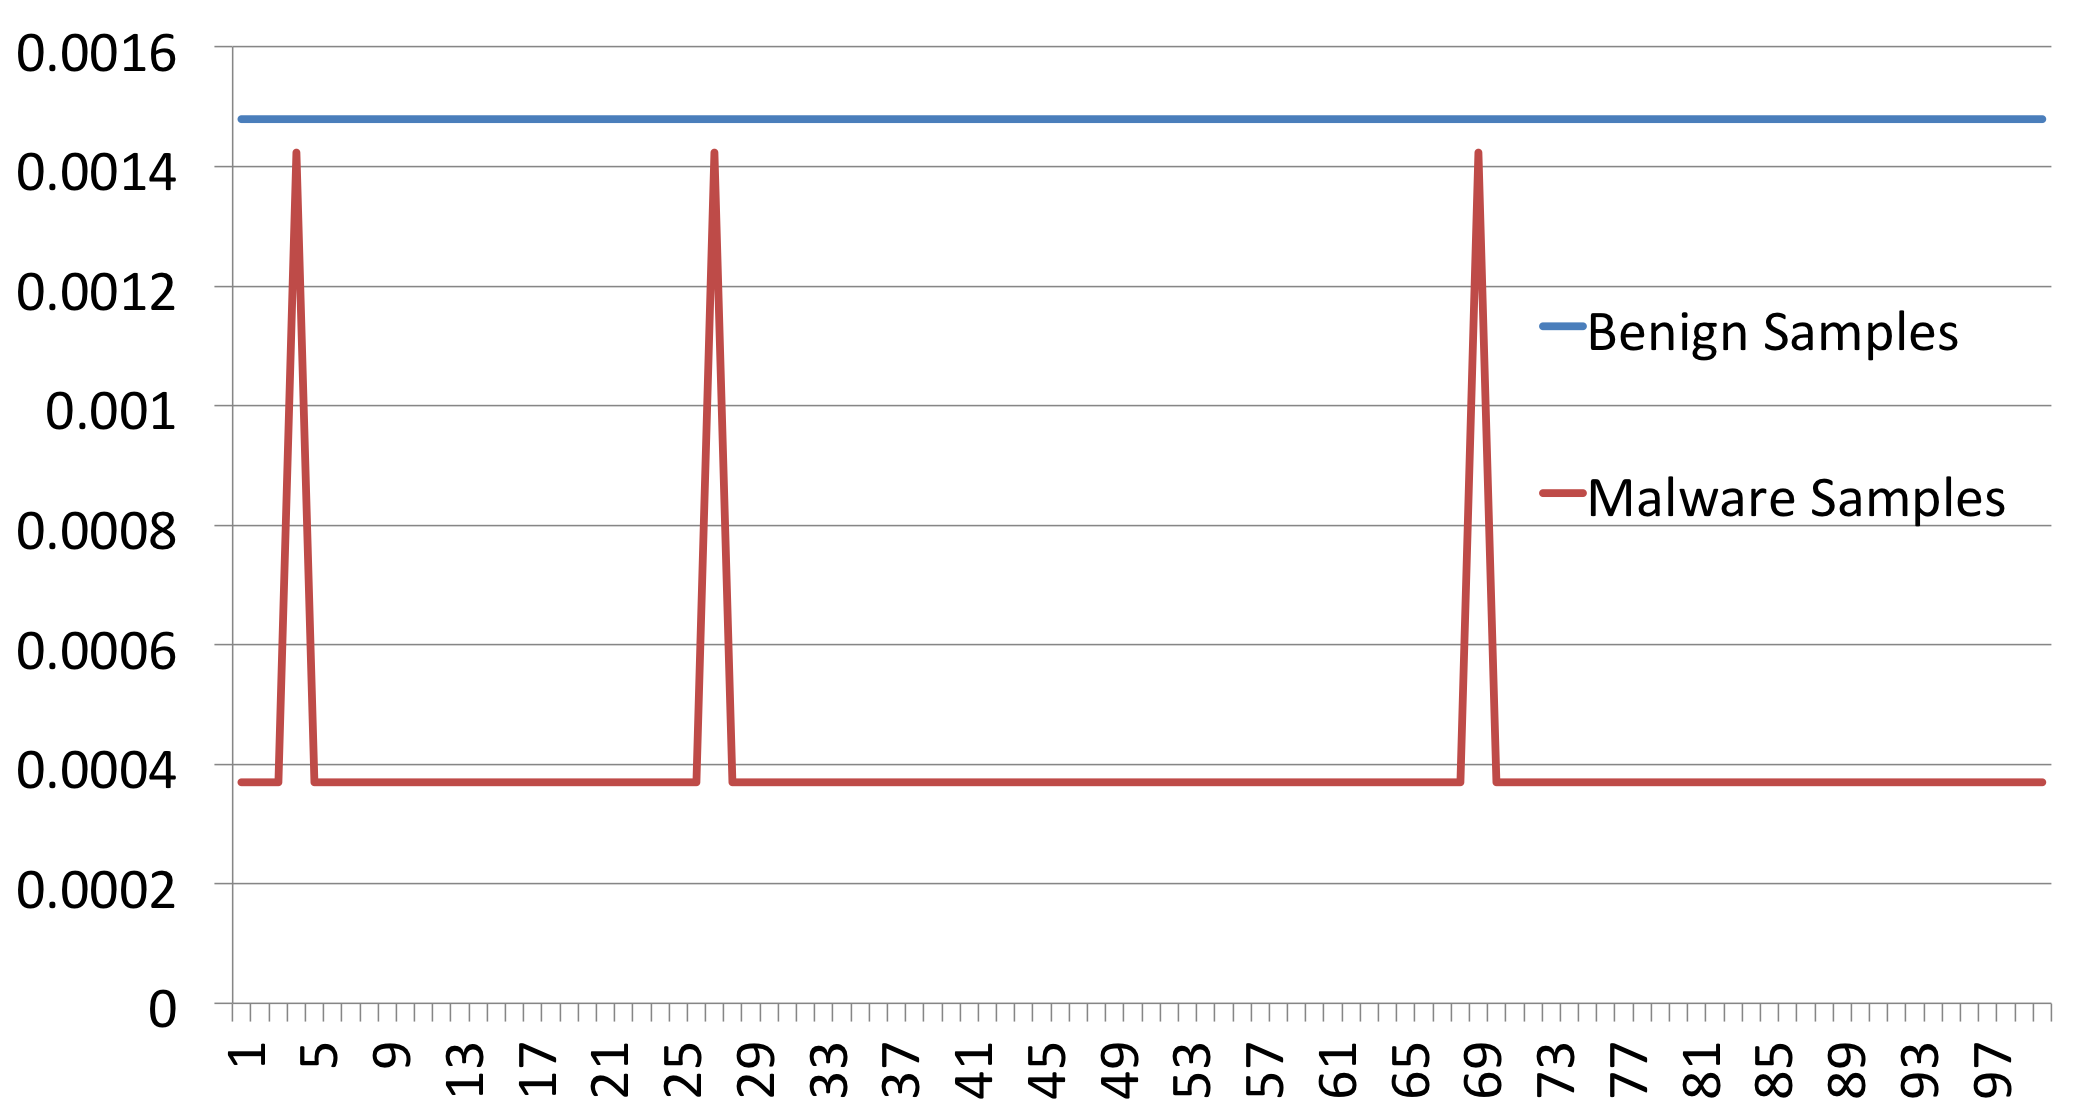
\includegraphics[width=8.4cm, height=10cm]{500.png}
	\caption{System Organization}
	\label{fig:systemorganization}
\end{figure}

\begin{enumerate}
	\item Packet Capture: This component takes care of capturing the packets and saving them into Packet Buffers. 
	\item Dissector: Dissector class consists of virtual functions, which is used to dissect the packet to obtain the attributes of the headers and the start of the payload. 
	\item Analysis: This component works on the GPU and performs header checking, pattern matching on the payload and works with the results.
\end{enumerate}

\section{Packet Capture}
The system defines PacketCapture as a class responsible for saving the packets into a packet buffer object. The BufferPacket class contains an array of packets, which contains the raw data from the network, the headers of the packets are stored. The size of the array is fixed and it should be easily accessible by the thread Index by the GPU. The kernel is launched with a specific number of threads based on the array size.
PacketCapture will obtain packets from one of the below mentioned modes and save them inside BufferPacket objects.
The two modes are:
\begin{enumerate}
	\item Live Capture mode: In this mode the system can capture the packets in real-time and use it for surveillance, anomaly prevention.
	\item Offline capture mode: In this mode, packets can be obtained from a tcpdump capture file or another source. They can be used to analyze and prevent a malicious attack in future.
\end{enumerate}
These classes use the LibPCAP library for capturing packets from a network interface card or a file. 

\section{Analysis}

Analysis is performed on the GPU using CUDA over the packet buffer objects.
The analysis module is divided into three components:
\begin{enumerate}
\item Auto-Mining: The entire packet analysis is divided among the threads. Each thread requires the data before it could perform the analysis. As already mentioned the shared memory is much faster than global memory. So the data required for each thread is saved in the shared memory in this module.
\item Operations: In this module the threads operate on the collected data. Header checking and pattern matching is implemented. Naive algorithm and Rabin Karp algorithm are used for pattern matching. The results are written into an array after the rules are checked.
\item Hooks: This module is written in C++. The results can be logged into a file or a database or they can be displayed on the screen. Libmysqlclient is the library used to communicate with the database.	
\end{enumerate}

\section{Parallelism approaches}

There are two types of parallelism employed to speed up packet processing on the GPU as shown in Figure ~\ref{fig:thread level} and Figure ~\ref{fig:block level}. In thread-level parallelism every packet is handled by a single thread. The kernel is launched with 96 blocks of 128 threads each. Each thread works on multiple rules; header checking and pattern matching. The code was optimized to use shared memory. Naive pattern matching was the first version of signature matching implemented.The patterns are stored in global memory. We found that in Naive pattern matching each thread was accessing the global memory N times, where N is the number of patterns X maximum pattern length. The time taken to access data from the global memory is approximately 200 to 300 cycles. In order to decrease the global memory access, Rabin Karp algorithm was used. In Rabin Karp algorithm, each thread accesses the global memory M times, where M is the total number of patterns. We need not be concerned regarding the maximum pattern length, because only the pattern hash needs to be fetched from global memory.

To maximize the performance of the GPU, we proposed another approach to perform packet processing. In contrast to thread level parallelism, in block level parallelism a group of 128 threads process each packet. Kernel was launched with 208 blocks of 128 threads each. This entire block of threads work on the rules; such as header checking and pattern matching. In this approach, we encountered warp divergence. 

Warp divergence occurs when threads within the warp need to work on if conditions. When if conditions occur, the threads for which the if condition is not satisfied remain idle. To solve this problem we modified the code such that threads in different warps execute different if conditions. Threads in Warp 1 execute the IP rules, threads in Warp 2 execute the TCP rules, threads in the remaining warp execute pattern matching.

\begin{figure}
	\centering
	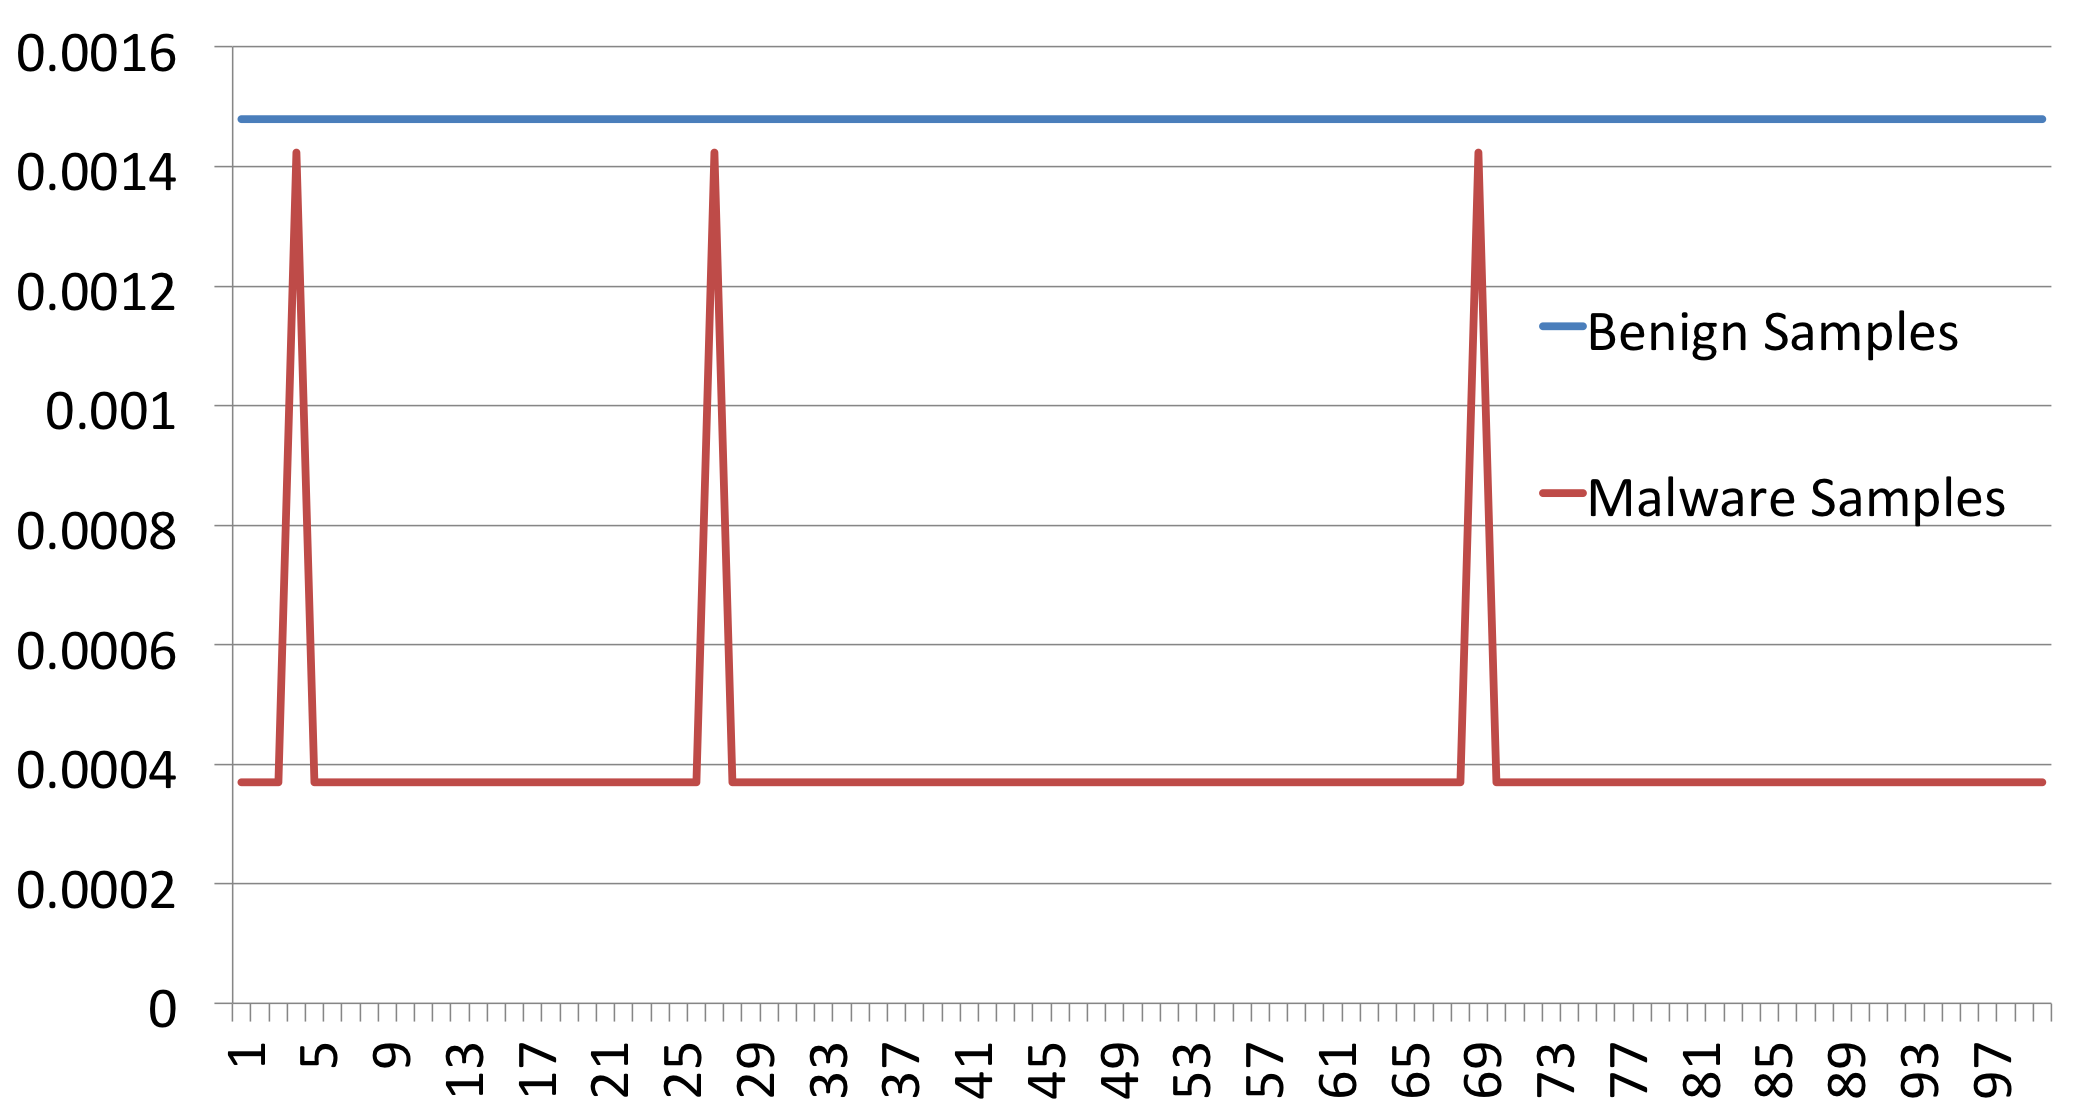
\includegraphics[width=8.4cm, height=10cm]{500.png}
	\caption{[a different packet is processed by each thread, each SP searches independently.]Thread Level Parallelism}
	\label{fig:thread level}
\end{figure}

\begin{figure}
	\centering
	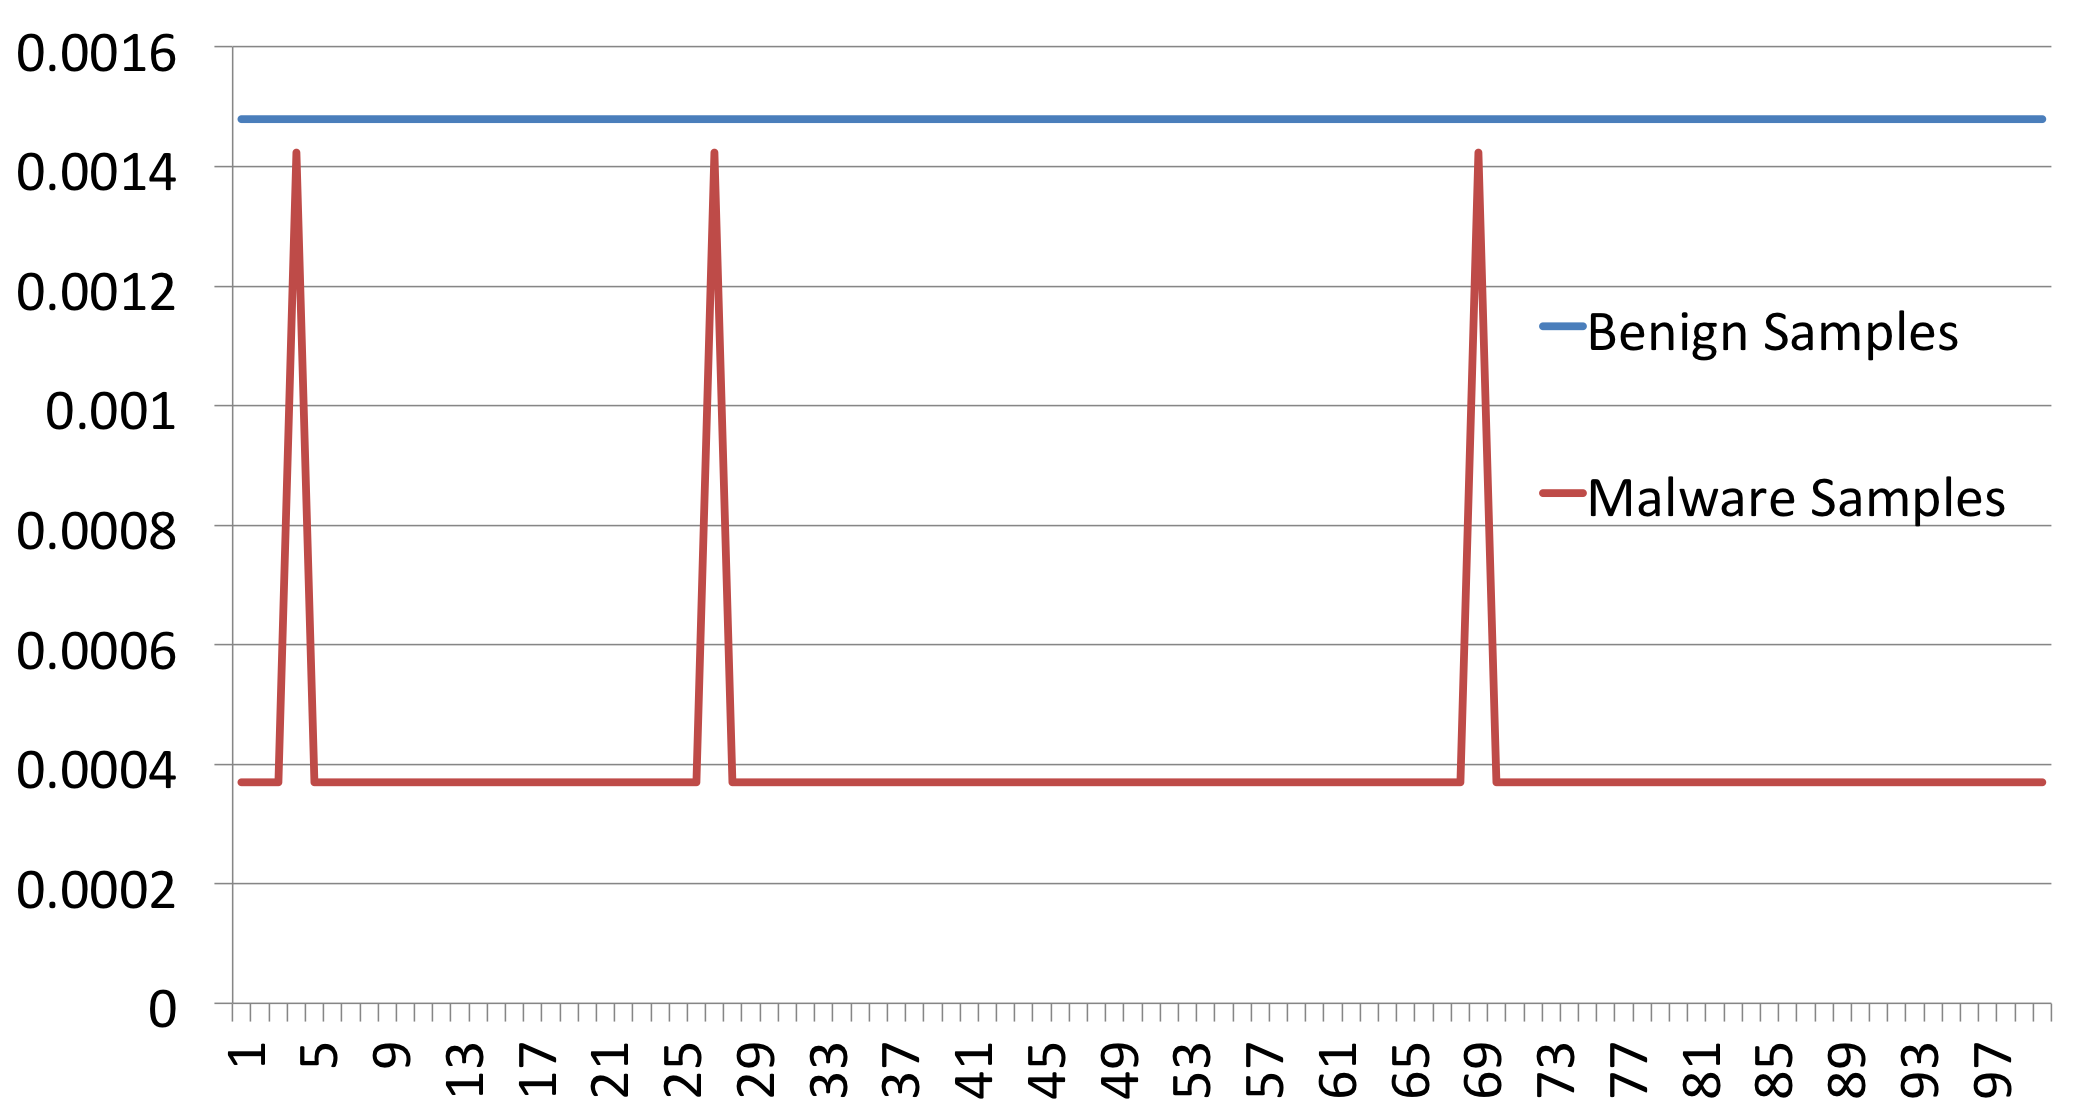
\includegraphics[width=8.4cm, height=10cm]{500.png}
	\caption{[a different packet is processed by each block. All the SP’s(Streaming Processor’s) search together.]Block Level Parallelism}
	\label{fig:block level}
\end{figure}

The next two sections explain in detail Header checking and Pattern Matching executed by the threads.

\section{Header Checking}
An attacker will send crafted packets to a computer to consume all its resources such that it cannot service any other request. The headers of the packets were analyzed by applying certain rules on them. 

The rules are:
\begin{enumerate}
	\item
	Check if the IP address of the packet is in the private address range because there can be no computer in the internet whose IP address is in this range.
	\item
	Check if the flag bits in the TCP header can be crafted or check if the reserved bits are set. For ex: it is not possible to have a combination of the SYN and FIN bit set.
	\item
	Check if the acknowledgement bit is set and the acknowledgement number is zero. Check if the source or destination port is zero for a TCP packet.
	\item
	Check if the IPv4 checksum can be tampered while in transit.
	If any of the above rule matches, the packet is discarded from further processing
\end{enumerate}

\section{Signature matching}
Naive algorithm was used to implement single pattern matching and Rabin Karp algorithm was used to implement both single pattern matching and multi-pattern matching. In the naive algorithm each thread starts searching from a specific byte number which corresponds to its index. For ex: thread 0 starts searching from byte 0, thread 1 starts searching from byte 1 and so on. Each thread searches up to the pattern length starting from its byte. If there is a match the results are updated.

In the Rabin Karp algorithm every thread computes the hash code for the payload it operates on and compares with the hashcode of the pattern. In the CPU version rabin karp algorithm, the hash codes can be computed for the neighbouring values, by using the previously computed hash code and adding only the extra character. Thus the run time complexity for checking if the hashcode of the pattern exists in the payload in linear. But this cannot be done on the GPU because all the threads are executing in parallel. So all the threads compute the hash code up to the pattern length and compare with the hash code of the pattern. The hash codes of the patterns are computed by a single thread at the same time when the header checking is done by the other threads. If the patterns are stored in global memory, then the Rabin Karp algorithm has very high performance when compared to the naive algorithm. In Rabin Karp algorithm for n threads, only once the global memory is accessed for comparing the pattern hashes; but in naive algorithm the global memory is accessed n times to compare the pattern and the payload.

The single pattern Rabin Karp algorithm is modified to obtain the multi-pattern searching algorithm. In the multi-pattern matching version, the patterns are represented by a two-dimensional array. In order to copy the two-dimensional array to the GPU, the two dimensional array is flattened to obtain a one dimensional array, which is then copied to the GPU. Every thread starts comparing the hashcode of every pattern to the payload from the byte corresponding to its thread Index. Multiple iterations are run by each thread corresponding to the number of patterns. 